\documentclass{article}

%other packages
\usepackage[a4paper]{geometry}
\usepackage{longtable}
\usepackage{wrapfig}
\setlength\parindent{0pt}
\usepackage{enumitem}
\usepackage[table,dvipsnames]{xcolor}
\usepackage{polynom}
\def\scaleint#1{\vcenter{\hbox{\scaleto[3ex]{\displaystyle\int}{#1}}}}
\usepackage{array}
\newcolumntype{C}{>{{}}c<{{}}} % for '+' and '-' symbols
\newcolumntype{R}{>{\displaystyle}r} % automatic display-style math mode 
\usepackage{tabularray}
\usepackage{dcolumn,tabularx,booktabs}
\usepackage[most]{tcolorbox}

%maths
\usepackage{mathtools}
\usepackage{amsmath}
\usepackage{amssymb}
\usepackage{amsfonts}
\usepackage{autobreak}

%tikzpicture
\usepackage{tikz}
\usepackage{scalerel}
\usepackage{pict2e}
\usepackage{tkz-euclide}
\usepackage{tikz-3dplot}
\usetikzlibrary{calc}
\usetikzlibrary{patterns,arrows.meta}
\usetikzlibrary{shadows}
\usetikzlibrary{external}
\usetikzlibrary{decorations.pathreplacing,angles,quotes}

%pgfplots
\usepackage{pgfplots}
\pgfplotsset{compat=1.18}
\usepgfplotslibrary{statistics}
\usepgfplotslibrary{fillbetween}

\pgfplotsset{
    standard/.style={
    axis line style = thick,
    trig format=deg,
    enlargelimits,
    axis x line=middle,
    axis y line=middle,
    enlarge x limits=0.15,
    enlarge y limits=0.15,
    every axis x label/.style={at={(current axis.right of origin)},anchor=north west},
    every axis y label/.style={at={(current axis.above origin)},anchor=south east}
    }
}

\begin{document}

Math 115 - Related Rates - 28 Jan 2024
\hrule

\vspace{10pt}

As I said in the email, Stewart's textbook does not properly introduce the intuition for solving related rates problems - he appears to be out of touch with student psychology in this regard. I will correct this for you.

\vspace{10pt}

Let's start off with something very simple. Given the formula $ab=cd+ef$, solve for $a$. Easy right? The answer is just $a=(cf+ef)/b$, which we know from basic algebra.

\vspace{10pt}

Related rates problems seem hard at first glance, but all they do is give you enough information to plug right into a formula like the one above - and - BAM! - there's your answer. 

\vspace{10pt}

The whole goal of the problem is just to find what that formula is. In the context of related rates problems, we are dealing with rates of change of certain quantities when they are at known values;  this means we need a formula that contains these quantities, as well as their derivatives. This is done by taking a formula which relates the quanntities (without their derivatives), and implicitly differentiating it with respect to time to obtain a formula which does contain the derivatives.

\vspace{10pt}

In the case of a right triangle, we may be given a side length, an angle, and a rate. 

\vspace{10pt}

{\bf{}EXAMPLE} Find the rate of change of the horizontal projection of an air-plane - ascending at an angle $\alpha$ - who'se hypotenuse is changing at a constant rate of $m\mbox{ km/h}$, where the hypotenuse equals a constant: $h=C\mbox{ km}$.

\begin{center}
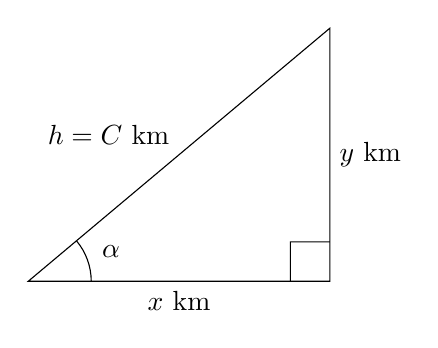
\begin{tikzpicture}[scale=5]
\coordinate (O) at (0,0);
\coordinate (P) at (40:1);
\coordinate (X) at (P |- O);

\draw[] (O) -- node[pos=0.5,above left]{$h=C\mbox{ km}$} (P) -- node[pos=0.5,right]{$y\mbox{ km}$} (X) -- node[pos=0.5,below]{$x\mbox{ km}$} cycle;

\draw pic["$\alpha$",draw,-,angle eccentricity=1.4, angle radius=0.8cm]{angle=X--O--P};
\draw pic["",draw,-,angle eccentricity=1.4, angle radius=0.5cm]{right angle=P--X--O};
\end{tikzpicture}
\hspace{30pt}
\raisebox{45pt}{where $\frac{dh}{dt}=m\mbox{ km/h}$}
\end{center}

\vspace{10pt}

\underline{WANTED} (dead or alive, lol): $\quad\frac{dx}{dt}\mbox{ such that }h=C$

\vspace{10pt}

I will show you a much shorter solution after the general solution; that being said, it's useful to understand the general solution. There is also a way to simplify the general solution (by substituting $C$ for $h$ half-way though, but I won't do that because I want you to see the general process for arbitrary variables - this will be more educational.

\vspace{10pt}

\underline{SOLUTION 1}:

\vspace{10pt}

First we \textit{relate} the non-derivative variables: $h^2=x^2+y^2$

\vspace{10pt}

Next we differentiate both sides with respect to time: $2x\frac{dx}{dt}+2y\frac{dy}{dt}=2h\frac{dh}{dt}$

\vspace{10pt}

Here we \textit{could} cancel the 2's and substitute $C$ for $h$, but I won't because of the following wisdom: ``Give a man a fish, and he will be hungry again to-morrow; teach him to catch a fish, and he will be richer all his life."

\newpage

A common theme of related rates problems is the need to be aware of geometric properties of the shape you are working with. For instance, in the case of right triangles, we can express the horizontal and vertical projections in terms of the angle and the hypotenuse - using the trig formulas. So,

\[2h\cos(\alpha)\frac{dx}{dt}+2h\sin(\alpha)\frac{dy}{dt}=2h\frac{dh}{dt}\]

\vspace{10pt}

Now we just solve for what we want and plug the values in - recall that since $y=h\sin(\alpha)$, we can re-espress it's derivative in terms of $h$; $\frac{dy}{dt}=\frac{d}{dt}h\sin(\alpha)=h^\prime\sin(\alpha)$:

\vspace{10pt}

(yes, I know that we could have just done this with the derivative of $x$ right at the very beginning, and this is the simpler solution I mentioned; but for reasons of teaching a person to fish, I chose to do it this way.)

\[\frac{dx}{dt}=\frac{2h\frac{dh}{dt}-2h\sin(\alpha)\cdot\left[\frac{dy}{dt}=\frac{dh}{dt}\sin(\alpha)\right]}{2h\cos(\alpha)}\]

\vspace{10pt}

Plugging in our values ($h=C;\quad\frac{dh}{dt}=m$), we arrive at thefollowing solution:

\[\frac{dx}{dt}=\frac{m-\sin\alpha\cdot m\sin\alpha}{\cos\alpha}=\frac{m(\cos^2\alpha)}{\cos\alpha}\overset{\therefore}{=}m\cos\alpha\]

\vspace{10pt}

And this is $100\%$ consistent with just doing it straight away with Pythagoras: $\frac{dx}{dt}=\frac{dh}{dt}\cos\alpha$

\vspace{10pt}

Hope this makes sense!


\end{document}
